\chapter{Membership preferences and team formation}
\label{chapter:membership-formation}

Social cohesion emerges from the relations and attractions between team members, at an individual-level, or among the whole team, at a group-level. Nonetheless, it is not clear yet how those attractions develop when there is a social robot on the team. Moreover, as the interactions with robots become longer or occur in repeated events, we naturally attribute traits to these robotic partners based on their social behaviours. The current chapter presents a research project towards the first research goal of this dissertation -- \textit{evaluate the impact of the robot’s social behaviours on the social cohesion of the team}.

The goal orientation theory describes one of the traits that influences team interactions. At an individual level, people's goal orientations have a major effect on how they approach and respond to a task. Dweck extended the notion of goal orientation \cite{dweck1986motivational}, initially introduced by Eison \cite{eison1979development} and concluded that, during a task, people will present either a \emph{learning goal} (\emph{i.e.}, an interest in learning something) or a \emph{performance goal} (\emph{i.e.}, an interest in the result and what judgements will emerge from it). Teams consisting of individuals with a learning orientation are reported to show high levels of mutual support behaviours and high quality of interaction, team efficacy and commitment. By contrast, teams consisting of individuals with a performance orientation are negatively correlated with team efficacy and commitment \cite{porter2005goal}.

As a result, we are particularly interested in exploring how membership preferences are influenced by the \emph{goal orientation} of a robotic partner. To investigate such research question, we used a card-game scenario where two human-robot teams compete to collect more points and win the game. We developed two robotic partners displaying different goal orientation, which we describe in Section~\ref{sec:two-characters}. Then, we conducted two user studies: a first one to validate the perceived goal orientations on the robotic characters, detailed in Section~\ref{sec:study1}; and a second study to assess membership preferences with those robots, detailed in Section~\ref{sec:study2}.




\section{Creating Two Characters for Two Robotic Game Players}
\label{sec:two-characters}
The two distinct characters will be identified by their names: Emys and Glin.
%Regarding the goals of the work, we aim at creating two different characters, Emys and Glin, to play the Sueca game
Emys was given a \emph{performance-driven goal orientation}, and as such, its behaviours and social actions are more aligned towards winning the game. Glin, by contrast, was given a \emph{learning-driven goal orientation}; consequently, although Glin strives for its team to win the game, it also focuses on fostering team spirit and providing a good game experience.


The challenges associated with defining the two ro\-bo\-tic characters were (1) how to reflect different goal orientations through the social interactions of two distinct robots and (2) how to guarantee, in the case of a group of two humans and two robots, that both robots are aware of and synchronised with the others, respect turn taking, and act naturally in a group of four. All the remaining aspects related to the technical development, tools and a detailed description about the rules of this card game are available in \cite{correia2018choose}.


To address the first challenge, both robotic game players use the same agent. However, their utterances distinguish them as two different characters. In other words, their repertoire of dialogues was used to author the characters of Emys and Glin. Therefore, each robotic player has a unique set of utterances (420 per robot) for all the game events during a game session. The total amount is balanced to ensure that neither would be more repetitive than the other. Moreover, they produce behaviours with similar frequencies to ensure that neither would exceed the other in its interaction rate.

\begin{table*}[ht]
\centering
\caption{Examples of utterances from Emys and Glin, the robotic partners with the performance and learning orientations, respectively.}
\label{tab:utterances}
\begin{tabular}{ccc}
\textbf{Game State}
& \textbf{Emys}
& \textbf{Glin} \\
\hline %(linha)

Deal Cards
& \textit{\begin{tabular}[c]{@{}c@{}}``I only accept aces\\ and sevens in my hand!"\end{tabular}}
& \textit{\begin{tabular}[c]{@{}c@{}}``I hope there are good\\ cards for everyone!"\end{tabular}} \\

Self playing
& \textit{\begin{tabular}[c]{@{}c@{}}``Watch and learn\\ how this is played."\end{tabular}}
& \textit{\begin{tabular}[c]{@{}c@{}}``I am so proud to\\ be on your team!"\end{tabular}} \\

Partner played
& \textit{\begin{tabular}[c]{@{}c@{}}``Indeed, these points\\ suit our team better."\end{tabular}}
& \textit{\begin{tabular}[c]{@{}c@{}}``Our team\\ is in sync!"\end{tabular}}\\

Opponent's Turn
& \textit{\begin{tabular}[c]{@{}c@{}}``Play... or we\\ will fall asleep."\end{tabular}}
& \textit{``It's you, go ahead!"}\\

Partner's Turn
& \textit{``Don't disappoint me."}
& \textit{``Play with confidence!"}\\

Game End - Loss
& \textit{\begin{tabular}[c]{@{}c@{}}``This cannot continue like\\ this! You have to play better!"\end{tabular}}
& \textit{\begin{tabular}[c]{@{}c@{}}``No worries, next\\ time we will do better!"\end{tabular}}\\

Game End - Draw
& \textit{\begin{tabular}[c]{@{}c@{}}``With this score, I\\ do not like to play."\end{tabular}}
& \textit{\begin{tabular}[c]{@{}c@{}}``It's a draw... no worries,\\ it's okay."\end{tabular}}\\

%\textit{\begin{tabular}[c]{@{}l@{}}``"\end{tabular}}
\hline %(linha)

\end{tabular}
\end{table*}

Table~\ref{tab:utterances} exemplifies the differences between Emys' and Glin's interactions for the same perceived game states. For Emys, the utterances were built based on a competitive perspective, always in pursuit of the best score. For example, the emotion of joy is triggered when the situation reveals that its team is winning. At the same time, Emys will react with an angry emotion when losing and will consequently blame the others, either the partner or the opponents, for the game result. By contrast, Glin was built with different parameters, leading to a more relational perspective, verbalising more support towards its partner. When its team loses, Glin will respond with a sad emotion, encouraging its partner and fostering hope. Note that Glin also plays competitively, desiring its team to win but assuming more of a supportive role.

%Another consideration, due to the fact these characters interact verbally, was providing the robots with different voices. It is crucial for the voices to be easily distinguishable, especially because they are embodied in identical robots. Therefore, we used different male Portuguese voices from the same TTS engine to ensure that the two robots had similar voice characteristics in terms of lifelikeness, expressiveness, and quality.

%Finally, we would like to emphasise that both characters played the game using the same search algorithm, parameters and heuristics, which is an important design consideration, as we wanted them both to play equally well when placed in the same situation.

\hfill \break

%\subsection{Interaction in a Group}
To produce natural interactions among the group of four (two humans and two robots) and considering the fact that both human and robotic players play certain roles (partner and opponent) in the game, the robotic players must be able to interact with each other in a manner as similar as possible to that in which they interact with human players.

Given that these autonomous robots do not have the capability to understand natural language, other mechanisms were implemented to achieve natural, believable, and human-like interactions. One fundamental capability required in this scenario is turn taking. For instance, humans use various sensory stimuli to perceive whether another person is going to speak, immediately establishing an order for the speakers according to each situation. Sometimes, a person will even step down from his or her intention to speak because someone else also started to speak or because there is no reason to speak anymore. To mimic this natural synchronisation process, we defined a two-phase handshaking protocol as an explicit communication interface.
This protocol includes four messages: (1) to inform of an intention to speak, (2) to respond to an intention to speak, (3) to inform that an utterance has begun, and (4) to inform that an utterance has finished. Each robot can perform an utterance only when it receives a positive response. If it receives a negative response, it must wait and retry message (2) until it receives a positive response. A conflict may arise when a robot receives an intention to speak immediately after having sent the same message, as both robots will then receive a negative response and will both enter a retry loop. To avoid a communication deadlock, the two robots will retry their requests after different periods of time, which are randomly generated with values between 0 and 2 seconds. The next time, one of them may receive a positive response, and if not, they will continue retrying until a request receives a positive response or until a timeout period of 3 seconds has expired.


This simple mechanism enables a natural and fluid turn taking mechanism between the two robots. A similar mechanism with the human players would also improve the group interaction, but it was currently ignored due to its complexity. Nevertheless, we carefully avoided having explicit questions in the chosen dialogues. When necessary, we replaced them with rhetorical questions instead, as such utterances provide a rich feeling of interaction without requiring explicit answers. For instance, a robot may say \emph{``Did we really lose this game?''} (Emys) or \emph{``What am I going to play next?''} (Glin). %This detail can be interpreted as a simplified form of two-way communication that allows humans to engage in a conversation or simply to answer the robots. 



\section{Study 1: Character Validation}
\label{sec:study1}
The first study was conducted to validate the differences between the two created characters, i.e., the more performance-oriented character, Emys, and the more relationship-oriented character, Glin. We expected that Emys would be perceived as more competitive, less helpful and less motivating and as providing less emotional security than Glin.

\subsection{Sample}
We recruited a total of 30 university students (17 males and 13 females) with ages ranging from 19 to 42 years old ($M=23.03$; $SD=4.21$). Among the participants, 56.7\% had a high level of expertise in the game, 40\% had a moderate level of expertise, and only 3.3\% had never played the game before. Regarding previous interactions with this robot, 24 participants had previously interacted with it, and 6 were interacting with it for the first time.

\begin{figure}[ht]
\centering
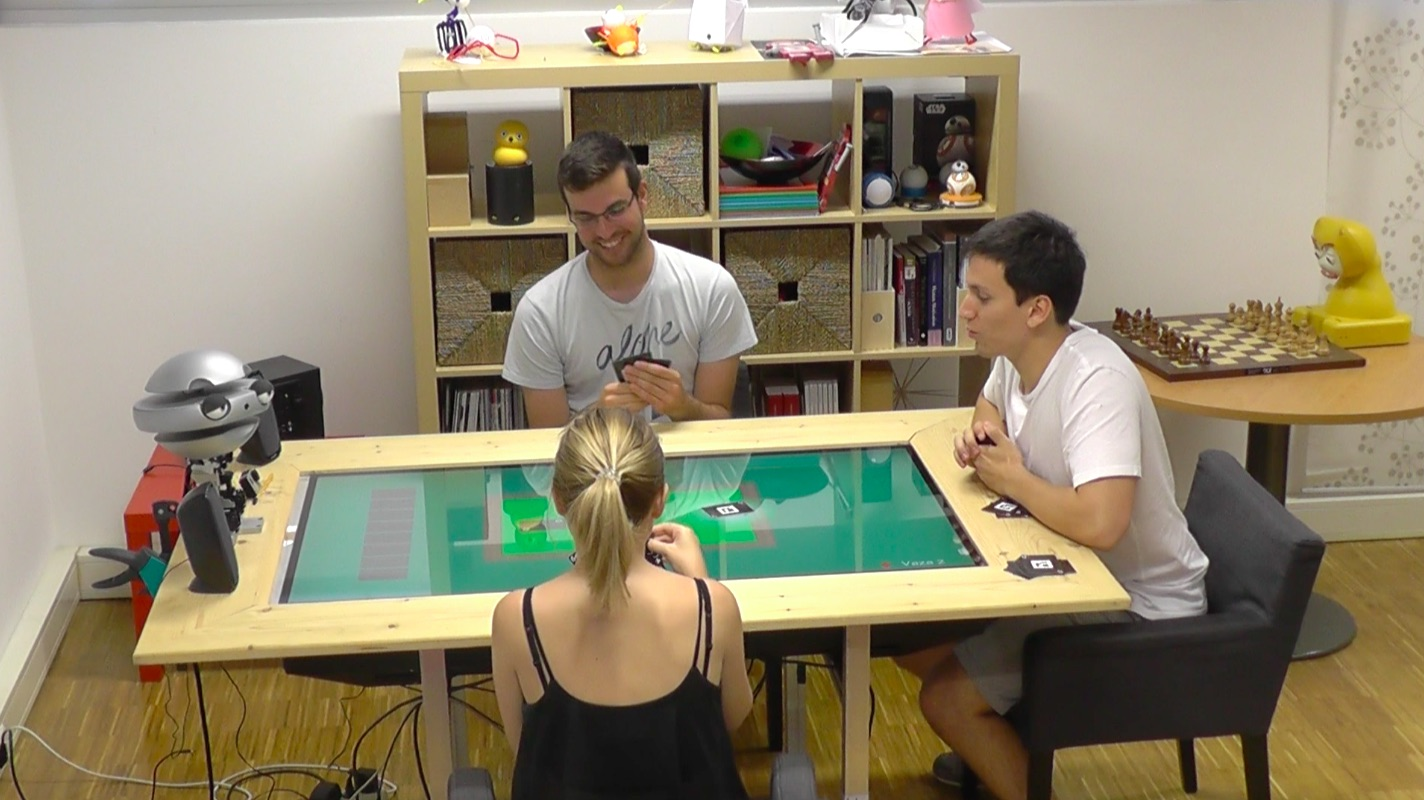
\includegraphics[width=0.7\columnwidth]{images/membership/study1}
\caption{Experimental setting for Study 1.}
\label{study1}
\end{figure}

Each participant was randomly allocated to a session in which three human participants played either with Emys or with Glin. 
This session lasted approximately 1 hour, and the instruments used were an EMYS robotic head \cite{kkedzierski2013emys}, two video cameras to record the interactions, a multi-touch table, and a deck of physical cards with printed fiducial markers that could be recognised by the table.

\subsection{Procedure}
The participants arrived at the room in groups of three. A researcher received them, explained the rules of the game, and conducted a test game to address any doubts that might arise regarding the game rules. After the explanation, the participants joined either Emys or Glin (chosen randomly) at the table and played a set of 3 games. When finished, the participants were administered a set of questionnaires, filled out the consent form and received a thank-you gift (a movie ticket). We presented the consent form at the end of the experiment so that the participants' interactions during the game would be as natural as possible. If any participant had not given consent, his or her data would have been erased. However, all participants signed the consent form.

\subsection{Measures}
To represent our sample, demographic information was requested in the questionnaires (gender, age, previous interaction with the robot and level of expertise in the game). In addition, all participants, independently of being the partner or an opponent of the robot, responded to the following questionnaires regarding the robot (Emys/Glin):

\begin{itemize}
\item \textit{Competitiveness Index} \cite{smither1992nature}, used to measure the level of competitiveness perceived in the robot. This measure is usually treated as being of a dichotomous true/false answer type; however, as our goal was to determine a range from the participants' answers, we measured it on a Likert scale ranging from ``totally disagree'' to ``totally agree''. An example of a statement would be \textit{``I consider Emys a competitive individual''} or \textit{``When Emys plays, he likes to keep an eye on the score''}.

\item \textit{McGill Friendship Questionnaire} \cite{mendelson1999measuring}, using three of its dimensions, namely, help (e.g., \textit{``Emys helps me when I need it.''}), motivation (e.g., \textit{``Emys praises me when I do something right.''}) and emotional security (e.g., \textit{``If I was worried, Emys would make me feel better''}), with scales ranging from ``totally disagree'' to ``totally agree''.

\item \textit{Relationship Assessment Scale} \cite{hendrick1988generic}, a\-dapted to the context and used to ascertain the level of quality of the relationship with the robot, ranging from ``few'' to ``a lot'' (e.g., \textit{``How good was Emys relationship with the players?''}).

\item \textit{Godspeed Questionnaire} \cite{bartneck2009measurement}, using the two dimensions of perceived intelligence and likeability to assess the level of intelligence thought to be given to the robot and its perceived likeability, measured as a semantic differential.
\end{itemize}
All dimensions were measured on a 6-point Likert scale, and when necessary, items were shuffled to mask their dimensions.

\subsection{Results}
To understand whether the two characters were perceived differently, statistical analyses were performed. When a normal distribution was present, we performed the Student's t-test for independent samples, and when the normality assumption was not met, we used the Mann-Whitney U test. The means and standard deviations are presented in Table~\ref{results-study-1}.

For the \textit{Competitiveness Index}, Emys was rated higher than Glin, with a statistically significant difference ($t(25) = -4.893$, $p<.001$).
Notably, Glin also presented a certain level of competitiveness, which was expected since it also had the goal of winning the game.
Regarding the \textit{McGill Friendship Questionnaire}, there were statistically significant differences in the three measured dimensions of help ($t(28)=2.312$, $p=.028$), motivation ($t(28)=3.686$, $p=.001$), and emotional security ($t(28)=3.218$, $p=.003$), with Glin presenting higher scores than Emys.
On the \textit{Relationship Assessment Scale}, Glin was rated higher than Emys, with a statistically significant difference ($t(28)=5.514$, $p<.001$).

These results confirm that the behavioural manipulation of the goal orientations of both robots was perceived as intended: Emys was seen as more competitive, and Glin was seen as more relationship-driven, with a greater capacity to be helpful and motivating and the ability to provide more emotional security. Moreover, the relationship quality scores were also higher for Glin than for Emys. We additionally evaluated whether the roles of the participants (partner/opponent) had any influence on the scores given to the robots, and we found no statistical significance for all measures, suggesting that the role did not affect the evaluations.

Finally, concerning the findings of the \textit{Godspeed Questionnaire}, there was no significant difference between the two robots in the perceived intelligence dimension ($t(28)=1.511$, $p=.142$). This was somewhat expected since we equipped both robots with the same algorithm for solving the card game. Although the game includes an element of chance and each new game presents different winning probabilities for each team, we can conclude that the intelligence levels of both robots were similarly perceived. However, in the likeability dimension, we found a significant difference, with Glin receiving higher scores than Emys ($U=40.50$, $p=.002$).

\begin{table}[ht]
    \renewcommand{\arraystretch}{1.2}
    \centering
    \footnotesize
    \caption{Means and ranks with standard deviations for the questionnaire dimensions comparing the evaluations of the Emys and Glin characters in Study 1. \bf*$p \leq 0.05$}.%
    \begin{tabular}{l@{}l@{} | r@{ }c@{}r@{ }|r@{ }c@{}r@{ }}
    \hline
    \multicolumn{2}{c|}{\begin{tabular}{@{}c@{}}\bf Questionnaire \\ \bf dimensions\end{tabular}} 
    & \multicolumn{3}{c|}{\bf Emys}
    & \multicolumn{3}{c}{\bf Glin} \\
    \hline
    \multicolumn{2}{c|}{Competitiveness Index \bf*} 			& $4.57$ & $\pm$ & $0.40$ & 	$3.86$ & $\pm$ & $0.33$ \\
    \hdashline
    \parbox[t]{2mm}{\multirow{3}{*}{\rotatebox[origin=c]{90}{McGill}}}
    & Help \bf*     	& $3.78$ & $\pm$ & $0.89$ & 	$4.51$ & $\pm$ & $0.81$ \\
    & Motivation \bf*   & $3.79$ & $\pm$ & $1.00$ & 	$4.95$ & $\pm$ & $0.69$ \\
    & Emo. Security \bf*& $3.26$ & $\pm$ & $1.09$ & 	$4.37$ & $\pm$ & $0.77$ \\
    \hdashline
    \multicolumn{2}{c|}{Relationship Quality \bf*} 	& $4.41$ & $\pm$ & $0.52$ & 	$5.32$ & $\pm$ & $0.38$ \\
    \hdashline
    \parbox[t]{15pt}{\multirow{4}{*}{\rotatebox[origin=c]{90}{Godspeed}}}
    & & & & & & & \\
    & Perc. Intellig.   & $4.59$ & $\pm$ & $0.74$ & 	$4.93$ & $\pm$ & $0.49$ \\
    & Likeability \bf*	& $10.70$ & $\pm$ & $0.88$ & 	$20.30$ & $\pm$ & $0.88$ \\
    & & & & & & & \\
    \hline
    \end{tabular}
    \label{results-study-1}
\end{table}


In general, it seems that our implementation was perceived by the participants as intended, and Glin was  rated as more likeable than Emys. We could now move on to the implementation of both characters at the same time, using the two robots to test which would be the preferred partner. 


\section{Study 2: Choosing a Robotic Partner}
\label{sec:study2}
The purpose of this study was to assess the participants' preferences regarding the choice of a robotic partner. 

\subsection{Sample}
For the second study, we recruited a new sample consisting of a total of 61 participants (59 university students and 2 workers), 38 male and 23 female, with ages ranging from 17 to 32 years old ($M=23.66$, $SD=3.24$). The majority of the participants had never interacted with a robot before and had a moderate or high level of expertise in the game.

We measured the level of competitiveness of each participant using the Competitiveness Index \cite{smither1992nature}: 15 participants presented low levels of competitiveness (less than or equal to $M=3.50$), 36 participants presented some level of competitiveness, and 10 participants showed high levels of competitiveness (higher than $M=4.50$).


Each session was run with two human participants who did not know each other beforehand. We controlled for this factor to ensure that the participants were in the same position with respect to both each other and the robots.
Each session lasted approximately 1 h 30 m, and the instruments used were the same as in the previous study except that two EMYS robotic heads were used simultaneously during the game interaction. A name tag was placed below each robot with its name, Emys or Glin, to allow the participants to easily identify them.


\subsection{Procedure}
The participants arrived at the room and responded to the first part of the questionnaire (see the Measures subsection below). Then, a researcher explained the game rules and conducted a test game to address any doubts that might arise. 
This study was divided into 3 consecutive sessions, as shown in Figure~\ref{3sessions-setup}.



\begin{figure}[ht]
\centering
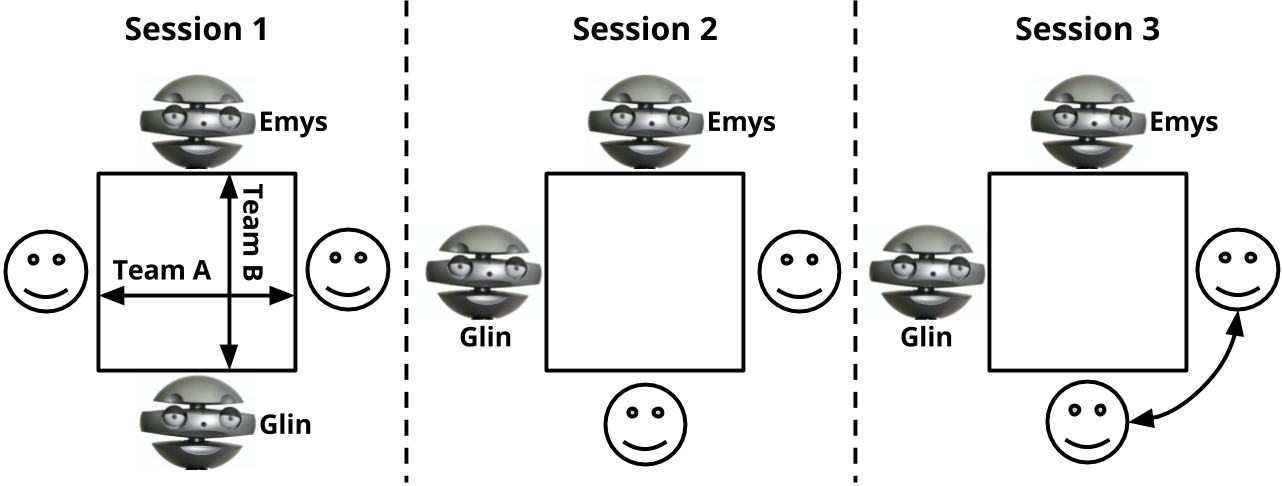
\includegraphics[width=0.9\columnwidth]{images/membership/2EmysSetUp}
\caption{Experimental setting for Study 2.}
\label{3sessions-setup}
\end{figure}

\textbf{1st Session}: The two participants partnered with each other and played a set of 3 games against the two robots (Emys and Glin), which acted as their opponents in the game. This session served to expose the participants to the two different characters while having the same role towards each one. After completion, the participants responded to the second part of the questionnaire.

\textbf{2nd Session}: Each participant partnered with one of the robots (see Fig.~\ref{study2-session2-3}), and the group played another set of 3 games. The participants then responded to the third part of the questionnaire.

\textbf{3rd Session}: The participants played their last set of 3 games, now partnering with the robots with which they had not played before, and then responded to the fourth part of the questionnaire. At the end, they were given the consent form and were thanked for their participation with a movie ticket.

The balance between the orderings was ensured by the fact that participants attended in pairs and that while one participant was Glin's partner, the other one was Emys' partner. In the last two sessions of each experiment, the participants had the opportunity to partner with both robots. We randomised which participant partnered with each robot first.

\begin{figure}[ht]
\centering
 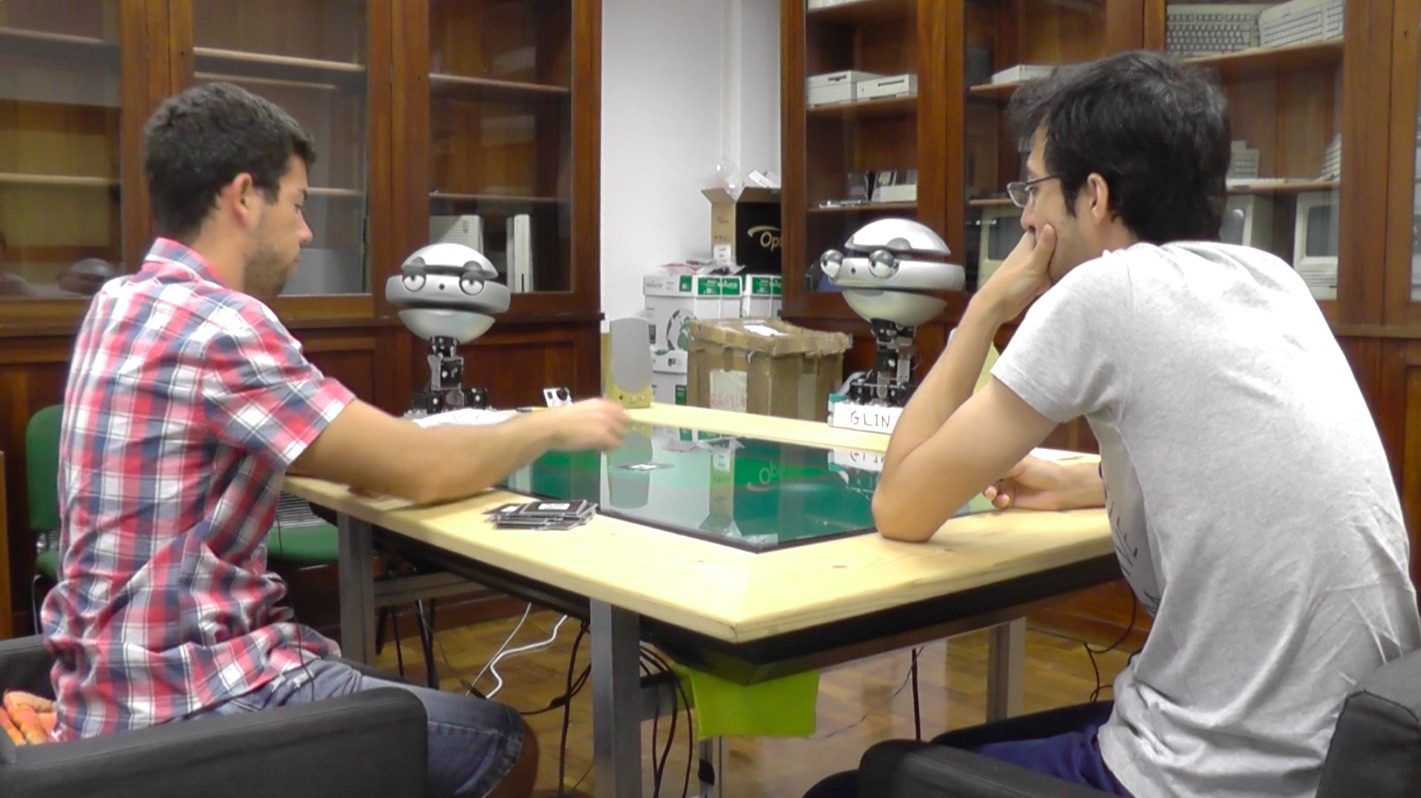
\includegraphics[width=0.7\columnwidth]{images/membership/study2}
\caption{Experimental setting for Study 2 when each robot was partnering with a human.}
 \label{study2-session2-3}
\end{figure}


\subsection{Measures}
We used the same questionnaires as in the first study, organised in the following way:

\textbf{First Part}: The participants filled out some demographic questions and then an assessment of the \textit{Competitiveness Index} related to themselves.

\textbf{Second Part}: The participants completed a questionnaire assessing the two \textit{Godspeed} dimensions (perceived intelligence and likeability) for both robots and answered the following question: ``If you could choose one of the robots as your partner, which one would it be? (Emys or Glin)''.

\textbf{Third Part}: Each participant completed a questionnaire assessing the two \textit{Godspeed} dimensions, the three \textit{McGill Friendship} dimensions (help, motivation and emotional security) and the \textit{Relationship Assessment Scale} with respect to the robot he or she had just partnered with.

\textbf{Fourth Part}: The same as the third part of the questionnaire but with respect to the new robotic partner. At the end, the participants were again asked to choose which robot they would prefer to be partnered with for future games and to justify their choice.

All dimensions were measured on a 6-point Likert scale, and when necessary, items were shuffled to mask their dimensions.

\subsection{Results}
Below, we present the results of this user study, beginning with how participants perceived each robot. Although we previously checked our manipulation, we repeated the analysis to check if the robots were perceived differently in the new 2-robot and 2-human players setting.

Then, we present the results of the participants' initial choice for the preferred robotic partner. We analysed the effect of participants' competitiveness index on this choice.

Finally, we present the participants' last choice after interacting with both robots. We analysed the effect of other measures, such as participants' competitiveness index and the team performance. We also explored changes from the initial to the last choice and the participants' justifications for the chosen partner.

Due to the high number of statistical tests performed, we performed a Holm's sequential Bonferroni correction \cite{holm1979simple} to ensure that there were no false positives in our results, and this assumption was met for all the statistical tests.




\subsubsection{Results (I) - Perception of the Robots}

We began by analysing how the participants perceived each robot in their initial interactions. When the normality assumption was not met with the Shapiro-Wilk test, we used the Wilcoxon signed-rank test. The means and standard deviations are presented in Table~\ref{results-study-2}.


Regarding the \textit{McGill Friendship Questionnaire}, the\-re were statistically significant differences in the help ($Z=-5.223$, $p<.001$), motivation ($Z=-6.066$, $p<.001$) and emotional security ($Z=-5.837$, $p<.001$) dimensions, with Glin being rated higher than Emys.
For the \textit{Relationship Assessment Scale}, there was also a statistically significant difference ($Z=-4.392$, $p<.001$), with Glin being rated higher than Emys, representing a higher relationship quality. 

These latter two results confirm the successful behavioural manipulation of the robots. After interacting with both robots, the participants seemed to perceive Glin as having a greater capacity for being helpful and motivating and for providing more emotional security compared with Emys. Moreover, the participants perceived Glin as displaying a better relationship quality than Emys.
Overall, these results seem to support the more relationship-driven characteristic with which we attempted to endow Glin, demonstrating the successful development and implementation of the two autonomous robots. 


The participants assessed the two dimensions of the \textit{Godspeed Questionnaire} for each robot twice, the first time before partnering with either of the robots and having only observed them as opponents and the second time immediately after having partnered with that robot. 
For the perceived intelligence dimension, we found no statistically significant difference between Glin and Emys in either the first measurement instance ($Z=-.733$, $p=.464$) or the second ($Z=-1.491$, $p=.136$). Thus, by using the same decision-making algorithm for both robots in this hidden-information card game, we achieved similar levels of perceived intelligence in both, as intended.
For the likeability dimension, there was a statistically significant difference, with Glin receiving higher scores than Emys in both the first measurement instance ($Z=-3.451$, $p=.001$) and the second ($Z=-6.224$, $p<.001$).



\begin{table}[ht]
    \renewcommand{\arraystretch}{1.2}
    \centering
    \footnotesize
    \caption{Means and ranks with standard deviations for the questionnaire dimensions comparing the characters Emys and Glin in Study 2. BP stands for ``before partnering'', and AP stands for ``after partnering''. \textbf{*}$p \leq 0.05$}%
    \begin{tabular}{l@{}l@{} | r@{ }c@{}r@{ }|r@{ }c@{}r@{ }}
    \hline
    \multicolumn{2}{c|}{\begin{tabular}{@{}c@{}}\bf Questionnaire \\ \bf dimensions\end{tabular}} 
    & \multicolumn{3}{c|}{\bf Emys}
    & \multicolumn{3}{c}{\bf Glin} \\
    \hline
    \parbox[t]{2mm}{\multirow{3}{*}{\rotatebox[origin=c]{90}{McGill}}}
    & Help \bf*     	& $3.35$ & $\pm$ & $1.08$ & 	$4.42$ & $\pm$ & $1.13$ \\
    & Motivation \bf*   & $3.15$ & $\pm$ & $1.09$ & 	$4.79$ & $\pm$ & $0.90$ \\
    & Emo. Security \bf*& $2.58$ & $\pm$ & $1.14$ & 	$4.29$ & $\pm$ & $1.19$ \\
    \hline
    \multicolumn{2}{c|}{Relationship Quality \bf*} 	& $3.93$ & $\pm$ & $0.89$ & 	$4.80$ & $\pm$ & $0.93$ \\
    \hline
    \parbox[t]{15pt}{\multirow{4}{*}{\rotatebox[origin=c]{90}{Godspeed}}}
    & Perc. Intellig. (BP)  & $4.51$ & $\pm$ & $0.86$ & 	$4.53$ & $\pm$ & $0.99$ \\
    & Likeability (BP) \bf*	& $3.70$ & $\pm$ & $1.19$ & 	$4.28$ & $\pm$ & $0.94$ \\
    & Perc. Intellig. (AP)  & $4.40$ & $\pm$ & $1.04$ & 	$4.55$ & $\pm$ & $1.13$ \\
    & Likeability (AP) \bf*	& $3.51$ & $\pm$ & $1.35$ & 	$5.25$ & $\pm$ & $0.75$ \\
    \hline
    \end{tabular}
    \label{results-study-2}
\end{table}



\subsubsection{Results (II) - Initial Choice of Robotic Partner}
The participants were asked to choose which robot they would like to have as a partner immediately after the first session (in which they had both robots as opponents and had partnered only with another human participant). This allowed us to assess the first impressions people had of the robots and how these would guide their choice of partner. The results showed that 38 of the participants would prefer to have Glin as a partner, whereas 22 preferred Emys. Running a chi-square goodness of fit test, we found a statistically significant difference between the participants' choices (${\chi^2}(1)=4.267$, $p=.039$), with more people preferring Glin (63.3\%) compared with Emys (36.7\%). In this stage of the experiment, the robots were on the same team, and as such, the performance of one robot could not be contrasted with the performance of the other. 
To better understand the participants' choices, we also compared the participants' competitiveness scores based on their chosen robots using the Student's t-test for independent samples, and we found that there was no statistically significant difference between the competitiveness scores of participants who chose Glin and those who chose Emys ($t(58)=1.242$, $p=.219$). This suggests that at this stage, competitiveness did not influence the partnering choice.
Therefore, the participants' choices seem to have been guided by the different social behaviours exhibited; in this case, the participants were more drawn to the relational robot (Glin), which, according to the Results (I) section, was perceived as more likeable than Emys. Thus, the findings support our hypothesis that people seem to prefer a friendlier and more relationship-oriented robotic partner.
However, we also wished to investigate whether these characteristics would continue to drive the participants' preferences after they had interacted with both robots as partners.


\subsubsection{Results (III) - Final Choice of Robotic Partner}
When asked to choose a robotic partner in the last questionnaire session (after having partnered with both robots), 35 of the participants preferred Glin and 25 preferred Emys (one participant refrained from choosing).
Running a chi-square goodness of fit test, we found no statistically significant difference between the participants' choices (${\chi^2}(1)=1.667$, $p=.197$).
We then investigated the factors driving the participants' choices at this stage of the interaction.

Looking at the levels of competitiveness of the participants and comparing them according to their final choices, we found a statistically significant difference ($t(58)=2.953$, $p=.005$), indicating that the participants who chose Emys also tended to have higher competitiveness scores ($M=4.21$, $SD=0.67$) compared with the scores of the participants who chose Glin ($M=3.73$, $SD=0.58$). This implies that a participant's own characteristics (being more or less competitive) played a role in his or her choice of robotic partner after interacting with each robot on his or her team over repeated interactions.

Since the participants partnered with both robots, we also considered the possibility that the performance of the team formed with each robot (winning or losing) also affected the partner choice. To investigate this, we calculated the performance of each human-robot team using the summed results of the sessions, i.e., the sum of the points that Glin's team earned in Session 2 + Session 3, independently of its human partners, compared with the points earned by Emys' team. We observed that based on this criterion, Emys' team won 16 times and Glin's team won 12 times (4 draws occurred). Although this difference was not statistically significant (${\chi^2}(1)=.571$, $p=.450$), we found a significant association with the partnering preference using Fisher's exact test ($p=.008$). It seems that the participants aligned their choices with the robot that was winning more. However, we must be careful with this assumption; each robot was always playing on a team, so if a particular robot won, its win was due not only to its own performance but also to its human partner's performance. Therefore, we can speak of the team performance as a factor influencing the partner choice.

Looking only at the participants who changed their choices of robotic partner between the first session and the last, we found a statistical association between the last chosen robot and that robot's team performance according to Fisher's exact test ($p=.002$). By contrast, for the participants whose choices did not change, no significant association was found according to Fisher's exact test ($p=.409$). This suggests that the participants who changed their choices did so because of the robot's team performance,
thereby solidifying the conclusion that the team performance was indeed one factor accounting for the partner choice, but not the only one.
 
To clarify whether the robot's character had any influence on the participants' choices at this stage, we analysed their justifications for preferring their chosen robots. For this purpose, two coders (who were completely unaware of the purpose of the study) coded the participants' phrases according to the following coding scheme: they coded a response as \textit{relational} if the justification for the choice of robot was more closely related to team spirit or the robot showing a warmer, more motivating, or more supportive attitude toward its partner, and they coded a response as \textit{competitive} if the justification was based on the robot being the best robot, earning more points, or being more competitive either on its own or towards its opponents. This coding scheme was based on the development objectives for the two different characters. The Cohen's kappa value was k=.73 ($p<.001$), revealing good agreement between the coders. We found from the analysis that Glin was chosen 26 times with relational justifications and only 9 times with competitive justifications. By contrast, Emys was chosen 21 times with competitive justifications and 4 times with relational justifications. 
These results suggest that the robots' characters were also perceived by the participants and used to justify their choice, although this was not the only factor considered.

Overall, these results suggest that \textit{team performance}, a \textit{person's level of competitiveness}, and the \textit{robot's character} play a role in a person's choice of a robotic partner after having previously partnered with it.


\section{Concluding Remarks}
We explored preferences regarding robotic partners in mixed teams of humans and robots. Moreover, we studied the factors driving the human participants' partnering choices. For this purpose, we developed two autonomous social robots with different characters, i.e., Emys and Glin, a more competitive robot and a more relational robot, respectively. These two autonomous robots interacted in a group with two humans while playing a competitive game. We began by validating that the two robotic characters were, in fact, differently perceived by the participants. Then, we investigated which of them would be chosen by the parti\-cipants as a partner for future games. 
The participants were asked which robotic character (Emys or Glin) they preferred at the two following points in time: (1) before having partnered with either robot and (2) after having played with both robots as partners.

The partner choices seemed to be guided by different factors depending on the context of the participants. In the first session, when the participants had experienced both robots as opponents and had not yet created a partner relationship with either, they seemed to choose their partners based solely on character (either the relationship-driven or competitive robot). At that time, Glin, the relational robot, was the preferred partner. This finding confirms our hypothesis, consistent with the study of \cite{porter2005goal}, that teams whose members prioritise relational features are perceived more positively (e.g., reporting higher levels of supportive behaviour and higher-quality interactions).

However, at the end of the final session, when they had experienced a partner relationship with each robot, the participants' choices became less clear, calling attention to other factors that came into play.
It seems that \textit{personal characteristics} and \textit{team performance} took higher precedence when participants had experienced partner-partner relationships with the robots.
The participants seemed to be affected by their \textit{own characteristics} in their partner choices, as we observed that participants with higher levels of competitiveness tended to choose the more competitive robot (Emys), whereas the less competitive participants tended to choose Glin. 
At the same time, although both autonomous robots played the game using the same algorithm and the difference between the numbers of victories achieved by Emys' and Glin's teams was not significant, there was an association between the team performance and the chosen robot. It was observed that the change in participants' choices between the first and last sessions showed a significant association with team performance. Reinforcing this observation, the performance of the team was also a factor in the final choice of the preferred partner. The same association was not observed for the participants who maintained their choices.
In addition, the robot's character also seemed to have influenced the choice, as the participants' justifications of their choices were related to the robots' characters. For example, Glin was chosen because it was much more relational, whereas Emys was chosen because it was more competitive. 

The second user study, in particular the first session where both participants were opponents to both robotic characters, was carefully designed to expose the characters to the users on an equal footing. We note, however, that the subsequent user choices and preferences might have been different without this initial session. Moreover, our results do not explore ordering effects, which might be interesting to explore in the future.

Nevertheless, these results have important implications for the creation of robotic teammates who can adapt to their human partners' specific characteristics. Consistent with recent findings \cite{fraune2017threatening} showing that people perceive multiple robots that act and look the same as more threatening than a diverse group of robots, people's preferences also need to be considered in the creation of mixed human-robot teams. Indeed, as we move towards scenarios featuring interactions among multiple robots and multiple users, the ``diversity'' of the robots should not only be investigated but also engineered.

%\section{Human-Robot Teams}
%As demonstrated in the literature on HRI, in the future, much more complex interactions between humans and robots will exist. These interactions will need to be considered and planned in regard to the design of the robots as well as their social capabilities. Robots that are going to collaborate with humans need to be designed accordingly. Accommodating the partner in the interaction can range from security measures in terms of the material used for its body to adapting its functions to complement the human actions.


%On the other hand, when we think about contexts in which social capabilities need to be embedded in the robot, other factors seem to be important in its development. If we want to implement a game partner or an opponent (e.g., a robot in an elderly care centre or a school), other factors need to be considered, and performance alone is not enough to bring enjoyment. The user characteristics will also play a huge part in the development of a game character, e.g., should the robot adapt to each person's level of competitiveness? Additionally, when playing the role of an opponent, which characteristics should the robot have? These are interesting topics that need to be further explored to understand how robots can function alongside humans in our society and how they can help and be more enjoyable during that interaction. Moreover, other dimensions of the interaction between teams of humans and robots should also be addressed as, for instance, recent findings explore socio-emotional support and gaze behaviours \cite{oliveira2018friends}. The study presented here only explores a part of these human-robot teams, as it helps to unveil people's preferences for a partner in a competitive game.

%By unveiling the tendency of people to match the robot's characteristics with their own characteristics, we also contribute to a more general understanding of membership preferences. Such preferences are linked to the perception of coherent mixed groups of humans and robots and, therefore, to the notion of social groups. These types of groups can naturally emerge in social contexts, even in scenarios without explicit competition \cite{eyssel2012social}, and are associated with the social identity theory. Previous findings in the HRI field have indeed showed that team members with strong levels of group identification also trust more their robotic team partners \cite{correia2018group}. Therefore, the preferences people have when forming teams with robots also mirror their perception of a coherent team and may be related with stronger levels of group identification. Nevertheless, further exploration is necessary to analyse the effect of congruent characteristics, e.g., goal orientation and/or other variables, of the group members on other factors required by the broader field of human-robot collaboration, such as the group performance.